\section{Durchführung}
\label{sec:Durchführung}

\subsection{Vorbereitung}
Zur Vorbereitung des Versuchs werden die Fourier-Koeffizienten von drei
verschieden periodischen Funktionen, in diesem Fall Rechteck-, Dreieck-,
und Sägezahn-Schwingungen, bestimmt. Dazu werden diese zur Vereinfachung so definiert,
dass es sich entweder nur um gerade oder ungerade Funktionen handelt.

\subsubsection{Rechteck-Schwingung}
\begin{figure}[H]
  \centering
  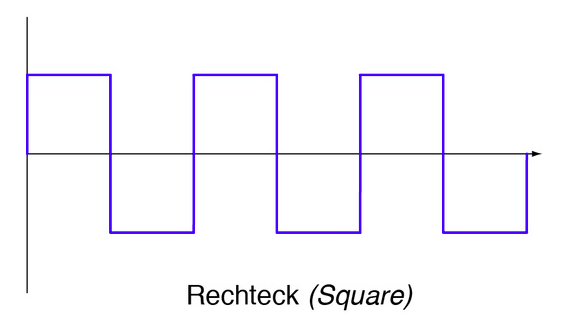
\includegraphics[height=7cm]{Rechteck.png}
  \caption{Rechteckschwingung \cite{Schwingungen}}
  \label{fig:reck}
\end{figure}
Definition:
\begin{equation}
  f(t)= \begin{cases}
         -A  , & -T < t < 0 \\
         A  , & 0 < t < T
      \end{cases}
\end{equation}
Da es sich um eine ungerade Funktion handelt, gilt $a_n = 0 $
\begin{align*}
  b_n &= \frac{1}{T} \int_{-T}^{T} f(t) \sin \left(\frac{n\pi}{T} t\right)dt \\
  &= \frac{2}{T} \int_0^T A \sin \left(\frac{n\pi}{T} t\right)dt \\
  &= \frac{2A}{n\pi} \left[-\cos \frac{n\pi}{T} t \right]^T_0 \\
  &= \frac{2A}{n\pi} (1-\cos (n\pi)) = \frac{2A}{n\pi}(1-(-1)^n) \\
  \implies b_n &= \begin{cases}
        0  , &\text{n gerade} \\
        \frac{4A}{n\pi} , &\text{n ungerade}
      \end{cases}
  \end{align*}

  \subsubsection{Dreieck-Schwingung}
  \begin{figure}[H]
    \centering
    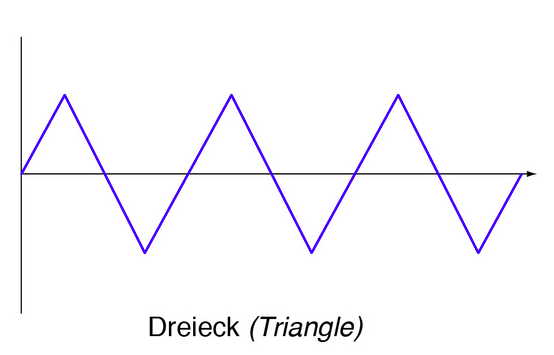
\includegraphics[height=7cm]{Dreieck.png}
    \caption{Dreieckschwingung \cite{Schwingungen}}
    \label{fig:deck}
  \end{figure}
  Definition:
  \begin{equation}
    f(t)= \begin{cases}
          \frac{2At}{T}   , & -T < t < 0 \\
          \frac{-2At}{T} , & 0 < t < T
        \end{cases}
  \end{equation}
  Da es sich um eine gerade Funktion handelt, gilt $ b_n = 0$
  \begin{align*}
    a_n &= \frac{1}{T} \int_{-T}^T f(t) \cos \left( \frac{n\pi}{T} t\right) dt \\
    &= \frac{1}{T} \int_{-T}^T f(t) \left(\frac{-2A}{T} \lvert t\rvert\right)
    \cos \left(\frac{n\pi}{T} t\right) dt \\
    &= \frac{2}{T} \int_0^T \frac{-2A}{T} t \cos \left(\frac{n\pi}{T} t\right) dt \\
    &= -\frac{4A}{T^2} \int_0^T \cos \left(\frac{n\pi}{T} t\right) t dt \\
    &= -\frac{4A}{T^2} \left(\left[\frac{Tt}{n\pi} \sin \left(\frac{n\pi}{T}t\right)\right]_0^T\right)
    - \frac{T}{n\pi} \int_0^T sin\left(\frac{n\pi}{T}t\right)dt \\
    &= -\frac{4A}{T^2} \left(\frac{-T^2}{(n\pi)^2}\left[-\cos\left(\frac{n\pi}{T}t\right)\right]\right) \\
    &= -\frac{4A}{(n\pi)^2} (cos(n\pi)-1) \\
    &= \frac{4A}{(n\pi)^2} ((-1)^n-1) \\
    \implies a_n &= \begin{cases}
          0  , &\text{n gerade} \\
          -\frac{2A}{(n\pi)^2}  , &\text{n ungerade}
        \end{cases}
\end{align*}

\subsubsection{Sägezahn-Schwingung}
\begin{figure}[H]
  \centering
  \includegraphics[height=7cm]{Saegezahn.png}
  \caption{Sägezahnschwingung \cite{Schwingungen}}
  \label{fig:säge}
\end{figure}
Definition:
\begin{equation}
  f(t)= \begin{cases}
        \frac{At}{T} - A  , & -T < t < 0 \\
        \frac{At}{T} , & 0 < t < T
      \end{cases}
\end{equation}
Da es sich um eine ungerade Funktion handelt, gilt $a_n = 0 $
\begin{align*}
  b_n &= \frac{1}{T} \int_{-T}^T f(t) \sin \left(\frac{n\pi}{T}t\right) dt \\
  &= \frac{-2A}{T^2} \int_0^T tsin\left( \frac{n\pi}{T}t\right) dt \\
  &= \frac{-2A}{T^2} \left[- \frac{tT}{n\pi} \cos \left(\frac{n\pi}{T}t\right)
  +\frac{T^2}{(n\pi)^2} \sin \left(\frac{n\pi}{T}t\right)\right]_0^T \\
  &= \frac{2A}{n\pi}(cos(n\pi)) \\
  &= \frac{2A}{n\pi}(-1)^n \\
  \implies b_n &= \begin{cases}
        \frac{2A}{n\pi}  , &\text{n gerade} \\
        \frac{-2A}{n\pi}  , &\text{n ungerade}
      \end{cases}
\end{align*}

\subsection{Fourier-Analyse}
Zur Durchführung der Fourier-Analyse wird an dem Funktionsgenerator
die zu analysierende Schwingung (Rechteck, Sägezahn
oder Dreieck) eingestellt und anschließend wird dieser
mit dem Oszilloskop verbunden. Dieses führt dann automatisch eine
Fouriertransformation durch, sodass die Amplituden und Frequenzen der einzelnen
$\delta$-Peaks mithilfe des Cursors ausgemessen und werden können. Diese Messung
wird für alle drei Schwingungsformen getrennt durchgeführt und die Messwerte
werden notiert. Der Versuchsaufbau ist in Abbildung \ref{fig:Aufbau} grob
skizziert.

\begin{figure}[H]
  \centering
  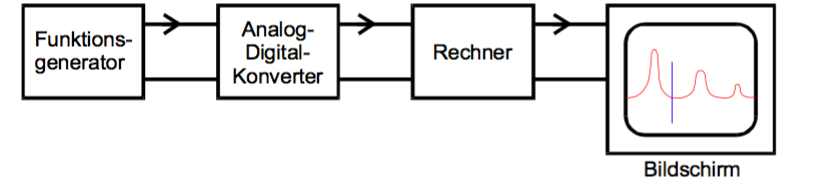
\includegraphics[width=15cm]{Aufbau.png}
  \caption{Versuchsaufbau \cite{skript}}
  \label{fig:Aufbau}
\end{figure}

\subsection{Fourier-Synthese}
Im zweiten Teil des Versuchs werden dann die in der Vorbereitung errechneten
Koeffizienten der Fourier-Reihe verwendet um die drei Spannungsformen aus
Sinusspannungen zusammenzusetzen. \\
Dazu wird das Oszilloskop in den X-Y-Betrieb geschaltet und mit je zwei
Ausgängen eines Oberwellengenerators verbunden. Mithilfe der Lissajous-Figuren
werden die beiden Ausgänge dann in Phase geschaltet. Anschließend wird einer der
beiden Ausgänge zusammen mit einem der anderen Ausgänge an das Oszilloskop
verbunden und dieser wird auf gleiche Weise erneut in Phase
geschaltet. Dieser Vorgang wird solange wiederholt bis alle Ausgänge phasengleich
sind. Dauraufhin wird das Oszilloskop zurück in den X-T-Betrieb gestellt und mit
dem Summationskanal des Oberwellengenerators verbunden, sodass die aufaddierten
Spannungen zu sehen sind. \\
Eventuell müssen die einzelnen Ausgänge dann noch um 180° variiert werden, bis
die entsprechende Funktion möglichst genau approximiert ist. Ist dies bis zu
einer ausrechenden Genauigkeit erfüllt, können die Ergebnisse mithilfe eines
Thermodrucks auf einem USB Stick gesichert werden.
